\documentclass[12pt,preprint]{aastex}
\usepackage{geometry}                % See geometry.pdf to learn the layout options. There are lots.
\geometry{letterpaper}                   % ... or a4paper or a5paper or ... 
%\geometry{landscape}                % Activate for for rotated page geometry
%\usepackage[parfill]{parskip}    % Activate to begin paragraphs with an empty line rather than an indent
\usepackage{graphicx}
\usepackage{amssymb}
\usepackage{epstopdf}
\usepackage{hyperref}
\DeclareGraphicsRule{.tif}{png}{.png}{`convert #1 `dirname #1`/`basename #1 .tif`.png}

\title{Planetary Astrophysics: Homework 3}
\author{Samuel Factor}
\date{\today}                                           % Activate to display a given date or no date

\begin{document}
\maketitle
Code for this assignment can be found at \url{https://github.com/sfxfactor/PlanetaryHW3}

\section{Part 1}
The method \texttt{calcF} in \texttt{diskModel} returns the flux density, $F_\nu$, of a star with temperature $T$, radius $R_s$, at a distance of $D_p$. A plot of the flux density of Fomalhaut at orbital radii of 10 and 130 AU is shown in Figure \ref{fig:FomFnu}. Stellar parameters are from \citet{Fom} ($T_\mathrm{eff}=8590$, $R_*=1.842 R_\odot$). 

\begin{figure}[htbp]
\begin{center}
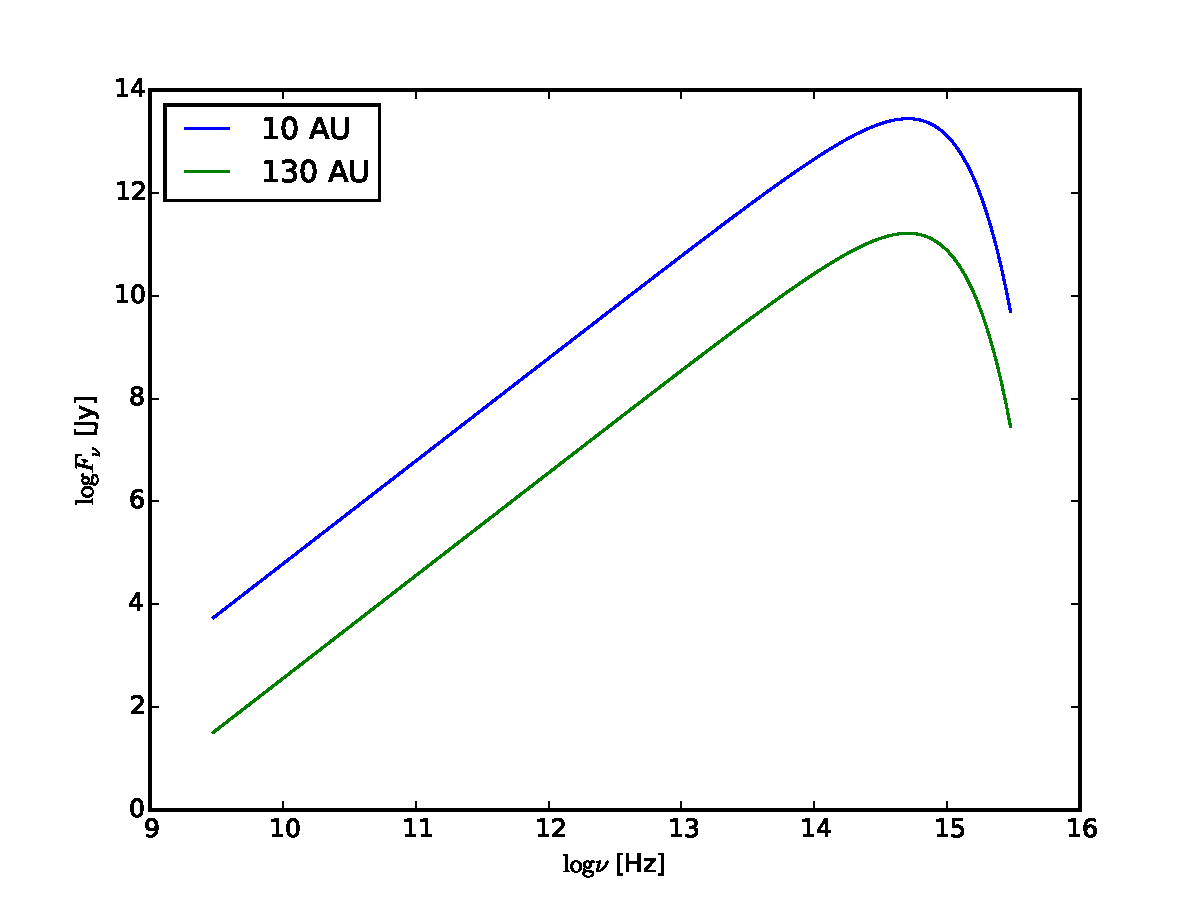
\includegraphics[width=0.8\textwidth]{FomFnu.pdf}
    \caption{Flux density of Fomalhaut}
    \label{fig:FomFnu}
\end{center}
\end{figure}

\section{Part 2}
The method \texttt{Pin} in \texttt{diskModel} returns the total power absorbed by a grain of radius $r_g$ [$\mu$m] and in a radiation field with flux density $F_\nu$. It first imports the $Q$ data obtained from the ``Smoothed UV Astronomical Silicate" models found at \url{http://www.astro.princeton.edu/~draine/dust/dust.diel.html} and extrapolates $Q_\mathrm{abs}$ to longer wavelengths with a $1/\lambda^2$ power-law. It then integrates, using the trapezoid rule the integral in Equation \ref{eq:Pin} from $\lambda=1$ cm -- 1 nm, where $r_g$ is now in cgs units.

\begin{equation}
P_\mathrm{in}=\pi r_g^2 \int Q_\mathrm{abs,\nu} F_\nu d\nu
\label{eq:Pin}
\end{equation}

$P_\mathrm{in}$ for different grain sizes, $r_g$ for different orbital radii $D_p$ are given in Table \ref{tab:Pin}.

\begin{table}[h]
\begin{center}
    \begin {tabular}{ccc}
    \tableline\tableline
    $r_g$ & $D_p$ [AU] & $P_\mathrm{in}$ [erg s$^{-1}$] \\
    \tableline
    0.1 $\mu$m & 10 & $1.46\times10^{-5}$\\
    1 $\mu$m & 10 & $6.25\times10^{-3}$\\
    10 $\mu$m & 10 & $6.61\times10^{-1}$\\
    1 mm & 10 & $7.13\times10^{3}$\\
    0.1 $\mu$m & 130 & $8.66\times10^{-8}$\\
    1 $\mu$m & 130 & $3.70\times10^{-5}$\\
    10 $\mu$m & 130 & $3.91\times10^{-3}$\\
    1 mm & 130 & $4.22\times10^{1}$\\
    \tableline
\end{tabular}
    \caption{$P_\mathrm{in}$ for Fomalhaut}\label{tab:Pin} 
\end{center}
\end{table}

\section{Part 3}
The method \texttt{Teq} in \texttt{diskModel} returns the equilibrium temperature of a grain of radius $r_g$ [$\mu$m] and incident power $P_\mathrm{in}$. Similar to \texttt{Pin}, it first imports the $Q$ data and extrapolates $Q_\mathrm{abs}$ to longer wavelengths with a $1/\lambda^2$ power-law. It then finds $T$ such that Equation \ref{eq:Teq}, where $B_\nu$ is the Planck function, is satisfied, using \texttt{scipy.optimize.root}. Again the integration uses the trapezoid rule. 

\begin{equation}
P_\mathrm{in}-4\pi^2 r_g^2 \int_{\lambda=1~\mathrm{cm}}^{\lambda=1~\mathrm{nm}} Q_\mathrm{abs,\nu} B_\nu(T) d\nu =0
\label{eq:Teq}
\end{equation}

The method \texttt{calcFQ} in \texttt{diskModel} returns the flux density, $F_\nu$ of a grain with temperature $T$, radius $r_g$, at a distance (from the observer) of D. Figures \ref{fig:Fnu10AU} and \ref{fig:Fnu130AU} show the flux density of a given set of grains at orbital radii of 10 and 130 AU, respectively, around Fomalhaut at a distance of 7.7 pc \cite{Fom}. The general trends of the flux densities make sense: smaller grains are fainter, as they have less surface area, but are hotter, as they are less like black-bodies. 

%\subsection{}

\begin{figure}[htbp]
\begin{center}
\includegraphics[width=0.8\textwidth]{Fnu10AU.pdf}
    \caption{Flux density of grains at 10 AU around Fomalhaut.}
    \label{fig:Fnu10AU}
\end{center}
\end{figure}

\begin{figure}[htbp]
\begin{center}
\includegraphics[width=0.8\textwidth]{Fnu130AU.pdf}
    \caption{Flux density of grains at 130 AU around Fomalhaut.}
    \label{fig:Fnu130AU}
\end{center}
\end{figure}

\section{Part 4}
An SED of Fomalhaut from \citet{SED} is shown in Figure \ref{fig:SED}. By scaling the peak flux density of the SED of a single grain up to the full SED, we can estimate the number of grains in the disk. If we then assume a density of 2 g cm$^{-3}$ we can also calculate a rough disk mass. These values are given in Table \ref{tab:mass} 

\begin{figure}[htbp]
\begin{center}
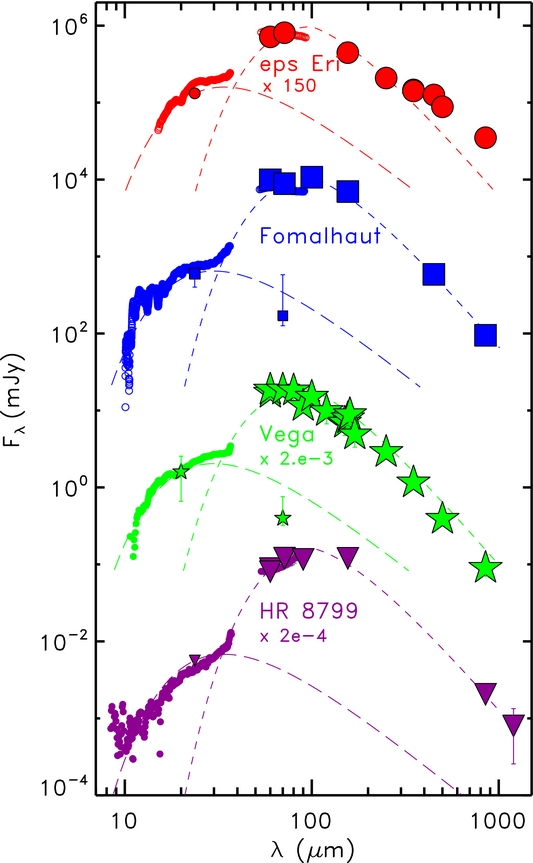
\includegraphics[width=0.5\textwidth]{apj455657f8_hr.jpg}
    \caption{SED of the two component disk around Fomalhaut from \citet{SED}.}
    \label{fig:SED}
\end{center}
\end{figure}

\begin{table}[h]
\begin{center}
    \begin {tabular}{cccc}
    \tableline\tableline
    $r_g$ & $D_p$ [AU] & $N$ & $M_\mathrm{dust}$ [g] \\
    \tableline
    0.1 $\mu$m & 10 & $5\times10^{26}$ & $4\times10^{12}$\\
    1 $\mu$m & 10 & $1\times10^{24}$ & $1\times10^{13}$\\
    10 $\mu$m & 10 & $9\times10^{21}$ & $7\times10^{13}$\\
    1 mm & 10 & $1\times10^{18}$ & $8\times10^{15}$\\
    0.1 $\mu$m & 130 & $9\times10^{29}$ & $7\times10^{15}$\\
    1 $\mu$m & 130 & $2\times10^{27}$ & $2\times10^{16}$\\
    10 $\mu$m & 130 & $6\times10^{24}$ & $5\times10^{16}$\\
    1 mm & 130 & $8\times10^{20}$ & $7\times10^{18}$\\
    \tableline
\end{tabular}
    \caption{Number of Grains and Dust Mass in Fomalhaut}\label{tab:mass} 
\end{center}
\end{table}

\section{Part 5}
Since we have already calculated the power absorbed by each grain it is simple to calculate the force due to radiation pressure ($F_\mathrm{rad}=P_\mathrm{in}/c$) and Poynting-Robertson drag ($F_\mathrm{pr}=P_\mathrm{in}\sqrt{GM_*/D}/c^2$, where $D$ is the orbital radius and $M_*$ is the mass of the central star). If we define $\beta=F_\mathrm{rad}/F_\mathrm{grav}$, we can calculate the characteristic timescale, $\tau$ in years, for dust grains to be removed from the system from Equation \ref{eq:time}, where $r$ is the initial orbital radius in AU and $M_*$ is the mass of the central star in $M_\odot$ \citep{beta}. These values are given in Table \ref{tab:forces}.

\begin{equation}
\tau=400\frac{r^2}{\beta M_*}
\label{eq:time}
\end{equation}

\begin{table}[h]
\begin{center}
    \begin {tabular}{cccccc}
    \tableline\tableline
    $r_g$ & $D_p$ [AU] & $F_\mathrm{rad}$ [dyn] & $F_\mathrm{pr}$ [dyn] & $\beta$ & $\tau$ [yr] \\
    \tableline
    0.1 $\mu$m & 10 & $4.9\times10^{-16}$ & $2.1\times10^{-20}$ & 5.1 & $4.1\times10^{3}$\\
    1 $\mu$m & 10 & $2.1\times10^{-13}$ & $9.1\times10^{-18}$ & 2.2 & $9.5\times10^{3}$\\
    10 $\mu$m & 10 & $2.2\times10^{-11}$ & $9.6\times10^{-16}$ & 0.23 & $9.0\times10^{4}$\\
    1 mm & 10 & $2.4\times10^{-7}$ & $1.0\times10^{-11}$ & $2.5\times10^{-3}$ & $8.4\times10^{6}$\\
    0.1 $\mu$m & 130 & $2.9\times10^{-18}$ & $3.5\times10^{-23}$ & 5.1 & $6.9\times10^{5}$\\
    1 $\mu$m & 130 & $1.2\times10^{-15}$ & $1.5\times10^{-20}$ & 2.2 & $1.6\times10^{6}$\\
    10 $\mu$m & 130 & $1.3\times10^{-13}$ & $1.6\times10^{-18}$ & 0.23 & $1.5\times10^{7}$\\
    1 mm & 130 & $1.4\times10^{-9}$ & $1.7\times10^{-14}$ & $2.5\times10^{-3}$ & $1.4\times10^{9}$\\
    \tableline
\end{tabular}
    \caption{Number of Grains and Dust Mass in Fomalhaut}\label{tab:forces} 
\end{center}
\end{table}

\bibliographystyle{apj}
\bibliography{sources}

\end{document}  
